\subsection{Dataset Statistics}

\begin{figure}[t]
    \centering
    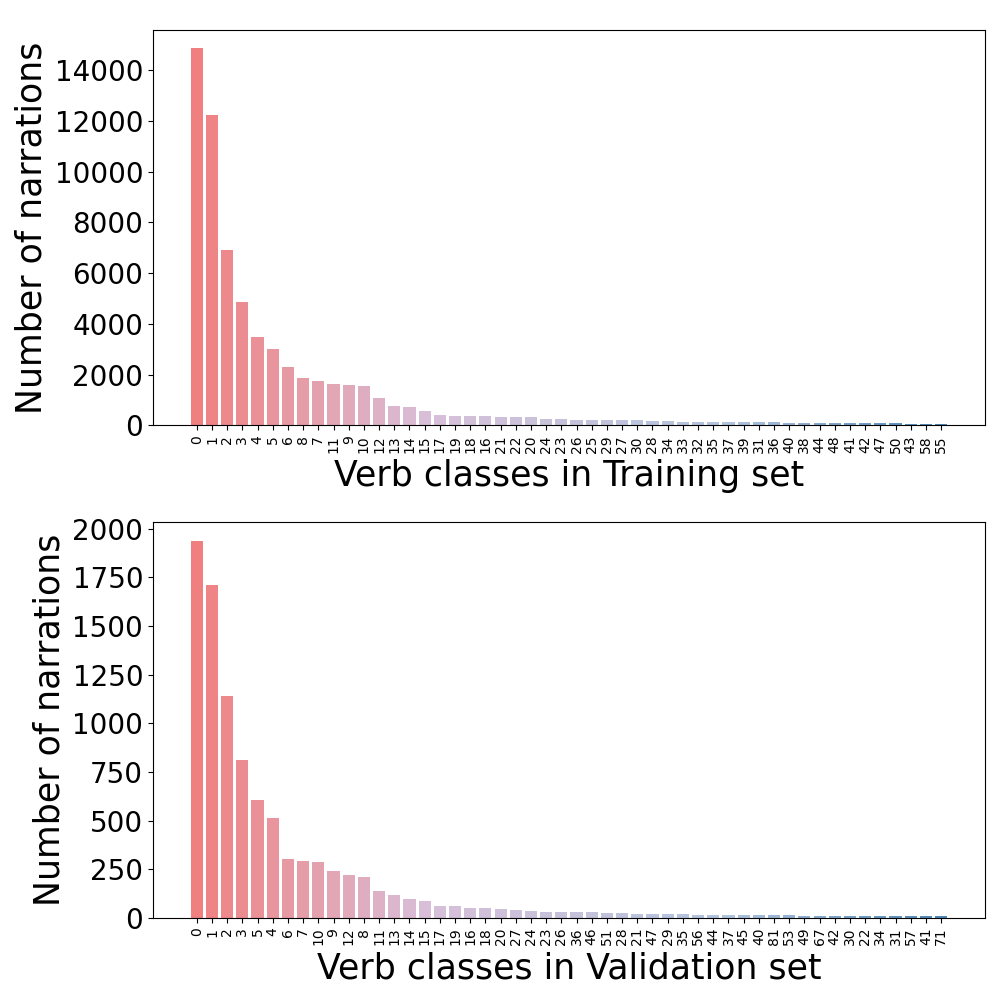
\includegraphics[scale=0.25]{figures/verb_count.png}
    \caption{Frequency distribution of 50 most frequent verb class in training and validation set}
    \label{fig:verb_freq}
\end{figure}

\subsubsection{Text Analysis}
Narrations in EPIC-KITCHENS-100 are mainly imperative phrases in the form of verb-noun with optional propositional phrase (e.g. \textit{put down plate}, \textit{put container on top of counter}). Each annotation includes start/stop timestamps and frames, action verbs and object nouns, which are extracted from the corresponding narration. Verbs and nouns are further classified into classes based on their semantic meaning. For example, \textit{grab} and \textit{get} belong to the same verb class.  There are a total of 97 verb classes and 300 noun classes in the training and validation set.

We define the frequency of a verb/noun class as the number of narrations that contain a verb/noun from that class. Both verb and noun classes have a heavy tailed distribution with tail classes ($\le$ 1/15 of the maximum frequency) accounting for 13.02$\%$ and 11.67$\%$ total verbs and 5.38$\%$ and 1.85$\%$ total nouns in the training and validation set respectively (Figure \ref{fig:verb_freq}). Such a distribution indicates the intrinsic complexity and entropy of the text data. The training and validation set have similar composition: in the validation set, there are no unseen verb class and only four unseen noun classes, accounting for 0.03$\%$ of all narrations. Narration timestamps are relatively complete: only 0.17$\%$ in training and 0.72$\%$ in validation are missing. On the other hand, since there were no constraints on the recording duration, we observe a great variability across videos. Average sentence length of training and validation set is 15.1 and 14.8 with standard deviation of 6.3 and 6.0 words, respectively. Average number of actions per video is 135.8 (training) and 70.1 (validation) with standard deviation of 167.7 and 93.2. More distribution statistics can be found in Appendix A Table \ref{table:train_val_stats}.

A natural assumption of our task is that there is none or minimal overlapping between action segments, i.e. only one action in almost all time frames. We check that there are at most 4 narrations in parallel in training and 3 in validation; only 3832 (5.70$\%$) and 617 (0.92$\%$) pairs of consecutive actions overlap for more than 1 second. We also inspect the feature embeddings of the verb and noun classes. Using GloVe word vectors pre-trained on Twitter (200d vectors) \cite{pennington2014glove}, we do not notice significant interclass or intraclass clustering effect (Appendix \ref{appendix:A} Figure \ref{fig:embedding}).

\begin{figure}[t!]
    % \begin{minipage}[b]{1\textwidth}
        \begin{subfigure}[b]{0.475\textwidth}
            \centering
            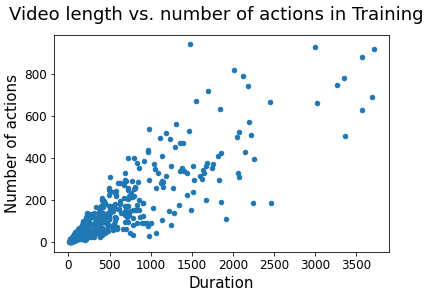
\includegraphics[scale=0.42]{figures/length_vs_actions_Training.png}
        \end{subfigure}\\
        \begin{subfigure}[b]{0.475\textwidth}
            \centering
            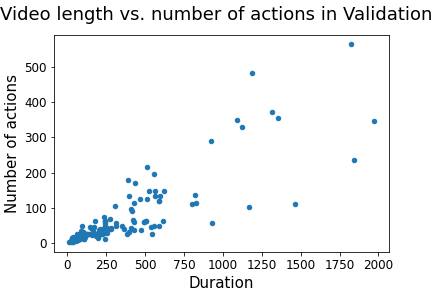
\includegraphics[scale=0.42]{figures/length_vs_actions_Validation.png}
        \end{subfigure}
        \caption{Number of action in each video against video length (in seconds)}
        \label{fig:action-freq-video-length}
    % \end{minipage}
\end{figure}

\subsubsection{Video Frame Analysis}
We extract 1920 $\times$ 1080 RGB frames from the videos at a sampling rate of 50 FPS. Each frame is identified by participant id, video id, and a start/end frame number. More than half of the total 700 videos in the dataset have less than 25,000 frames.  

Videos in EPIC-KITCHENS-100 have varied length with the longest video of 3708 seconds and shortest video of 10 seconds. 85.7 $\%$ of the videos are shorter than 1000 seconds and 66.0 $\%$ are less than 500 seconds (Appendix A Table \ref{table:train_val_stats}, Figure \ref{fig:duration}). 
%lacking sufficiency in support of longer videos.
% \cite{graphbased2020} mentioned that optimization tends to be slow for longer videos in action recognition tasks. 
We also see that the number of narrations grows roughly linearly with video length (Figure \ref{fig:action-freq-video-length}).  

%[Trim] If need to trim, we can trim on example words%
We compile all training and validation samples of a given verb class and compute the average number of frames for this class (Appendix Figure \ref{fig:avg-frame}). The top-10 verb classes with the most number of frames include actions like \textit{grate, wait, prepare, knead, stir}, and \textit{cut}; while those with the least number of frames contain actions like \textit{bend, turn-off, turn-on, take, close}. It seems that actions involved during cooking take longer than those related to intermediate preparatory steps, and the average length of the action aligns with how people would respond if asked about which action would take longer. For most verb classes, the average number of frames in each class are roughly the same in both training and validation set, except a few where the validation sets have more frames. We also count the total number of frames for each verb class, summed over all training and validation samples in the class. We notice that such frequency corresponds to the trend of verb-class frequency in the annotations (Appendix A Figure \ref{fig:total-frame}). This indicates that within the dataset, the frequency of the verb class correlates to the amount of visual information in the dataset.

The dataset also provides bounding-box annotations for each frame, where it only distinguishes between two categories: hands and objects. Only active objects are annotated, so the number of object bounding-boxes in a frame approximates the number of objects that the person interacts with. We compute the average number of hand bounding-boxes appearing in a frame of each verb class. Class with less than 1.5 hand bounding-boxes include actions like \textit{take, put-on, open, pull-down, walk}, and these correspond roughly to human impression on how many hands are needed for performing the action. We also compute the average number of objects bounding boxes in a frame of a given verb class. Verb classes with less than 1.8 object bounding boxes include actions like \textit{open, close, shake, check, fold}, and \textit{drink} (Appendix A Figure \ref{fig:hand-bbox}, \ref{fig:obj-bbox}). 
% \todo[inline]{Would be nice if we can generalize like more avg number of bounding boxes correlates to xx type of action?}
The average numbers of hand and object bounding boxes for the training and validation sets are mostly equal, despite the validation set misses a few verb classes. Full details can be found in Appendix \ref{appendix:A}.